\uuid{YouX}
\titre{Taille dans une population et probabilités}
\chapitre{Probabilité continue}
\niveau{L2}
\module{Probabilité et statistique}
\sousChapitre{Loi normale}
\theme{Loi normale, Variable aléatoire continue, Probabilités conditionnelles; Formule de Bayes}
\auteur{Grégoire Menet}
\datecreate{2025-05-07}
\organisation{AMSCC}

\difficulte{}
\contenu{
	
	\texte{
		Dans un pays, la taille en centimètres des femmes de 18 à 65 ans peut être modélisée par une variable aléatoire \(X_1\) suivant la loi normale d'espérance \(\mu_1 = 165\)\,cm et d'écart-type \(\sigma_1 = 6\)\,cm, et celle des hommes de 18 à 65 ans par une variable aléatoire \(X_2\) suivant la loi normale d'espérance \(\mu_2 = 175\)\,cm et d'écart-type \(\sigma_2 = 11\)\,cm.
		
		Dans cet exercice, tous les résultats seront arrondis à \(10^{-3}\) près.
	}
	
	\begin{enumerate}
		\item \question{Quelle est la probabilité qu'une femme choisie au hasard dans ce pays mesure entre $1{,}53$ m et $1{,}77$ m ?}
		\indication{Convertir les mesures en centimètres. Centrer et réduire la variable aléatoire $X_1$ pour utiliser la table de la loi normale standard ou les propriétés de la fonction de répartition.}
		\reponse{La taille d'une femme est modélisée par la v.a. $X_1$, qui suit la loi normale d'espérance $\mu_1 = 165$ cm et d'écart-type $\sigma_1 = 6$ cm.\\
			On convertit en cm : $1,53\,$m $= 153\,$cm et $1,77\,$m $= 177\,$cm. On cherche alors $P(153 \leq X_1 \leq 177)$.\\
			On a : $P(153 \leq X_1 \leq 177)= P\left(\frac{153-165}{6} \leq \frac{X_1-165}{6} \leq \frac{177-165}{6}\right)=P\left(-2 \leq \frac{X_1-165}{6} \leq 2\right)$.\\
			Si $Z = \frac{X_1-165}{6}$, alors $Z$ suit la loi normale centrée réduite.
			$P(-2 \leq Z \leq 2) = P(Z \leq 2) - P(Z < -2) = \Phi(2) - \Phi(-2)$.
			Comme $\Phi(-2) = 1 - \Phi(2)$, on a $P(-2 \leq Z \leq 2) = \Phi(2) - (1-\Phi(2)) = 2\Phi(2)-1$.
			Et grâce aux tables, on trouve : $P(153 \leq X_1 \leq 177)\simeq 0{,}954$.\\
}
		
		\item \question{Calculer la probabilité qu'un homme choisi au hasard dans ce pays mesure plus de $1{,}70$ m.}
		\indication{Centrer et réduire la variable aléatoire $X_2$. Exprimer la probabilité $P(X_2 \geq 170)$ en utilisant la fonction de répartition $\Phi$ de la loi normale centrée réduite.}
		\reponse{La taille d'un homme est modélisée par la v.a. $X_2$, qui suit la loi normale d'espérance $\mu_2 = 175$ cm et d'écart-type $\sigma_2 = 11$ cm.\\
			On cherche ici $P(X_2 \geq 170)$ (on applique un raisonnement similaire à la question 1 pour centrer et réduire $X_2$).\\
			$P(X_2 \geq 170) = P\left(\frac{X_2-\mu_2}{\sigma_2} \geq \frac{170-175}{11}\right) = P\left(Z \geq \frac{-5}{11}\right)$ où $Z$ suit la loi normale centrée réduite.\\
			$P(Z \geq -5/11) = P(Z \leq 5/11) = \Phi(5/11)$.
			On trouve grâce aux tables (ou à la calculatrice) : $P(X_2 \geq 170) \simeq 0{,}675$.}
		
		\item \question{On sait que dans ce pays les femmes représentent \(52\%\) de la population des personnes dont l'âge est compris entre 18 et 65 ans. On choisit au hasard une personne qui a entre 18 et 65 ans. Elle mesure plus de $1{,}70$ m. Quelle est la probabilité que cette personne soit une femme ?}
		\indication{Définir les événements $F$ (être une femme), $H$ (être un homme), et $C$ (mesurer plus de $1,70$ m). Calculer les probabilités conditionnelles $P(C|F)$ et $P(C|H)$ en utilisant la loi normale pour $X_1$ et $X_2$. Utiliser la formule des probabilités totales pour $P(C)$, puis la formule de Bayes pour trouver $P(F|C)$.}
		\reponse{Il s'agit d'un problème de probabilités conditionnelles.\\
			Soit $F$ l'événement : « La personne choisie est une femme ».\\
			Soit $H$ l'événement : « La personne choisie est un homme » (donc $H = \bar{F}$).\\
			Soit $C$ l'événement : « La personne choisie mesure plus de 1{,}70 m ».\\
			On sait que $P(F) = 0,52$, donc $P(H) = 1 - P(F) = 1 - 0{,}52 = 0{,}48$.\\
			On cherche la probabilité $P(F|C)$. D'après la formule de Bayes, $P(F|C) = \frac{P(C|F)P(F)}{P(C)}$.\\
			
			Calculons $P(C|F)$ : c'est la probabilité qu'une femme mesure plus de $1,70$ m, soit $P(X_1 \geq 170)$.\\
			$P(X_1 \geq 170) = P\left(\frac{X_1-165}{6} \geq \frac{170-165}{6}\right) = P(Z \geq 5/6)$.\\
			On trouve à la calculatrice (ou table) : $P(X_1 \geq 170) \simeq 0{,}202$. Donc $P(C|F) \simeq 0{,}202$.\\
			
			Calculons $P(C|H)$ : c'est la probabilité qu'un homme mesure plus de $1{,}70$ m, soit $P(X_2 \geq 170)$.\\
			Cette probabilité a été calculée dans la question 2 : $P(X_2 \geq 170) \simeq 0{,}675$. Donc $P(C|H) \simeq 0{,}675$.\\
			
			On peut représenter ces informations sur un arbre de probabilités :
			\begin{center}
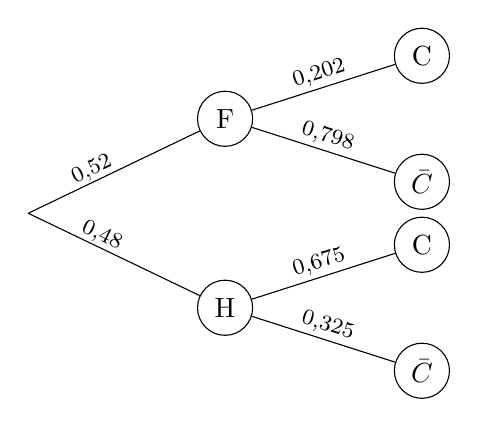
\begin{tikzpicture}[
	% Style for the nodes (circles)
	node_style/.style={
		circle,
		draw,
		minimum size=7mm, % Adjust size as needed
		inner sep=0pt
	},
	% Style for the probability labels on edges
	prob_style/.style={
		sloped, % Orients the text along the path
		midway, % Places it in the middle of the path
		above,  % Places it above the path (can be 'below')
		font=\footnotesize,
		inner sep=1.5pt % Small padding around text
	},
	% Define distances for tree layout
	level 1/.style={sibling distance=3cm},
	level 2/.style={sibling distance=2cm},
	edge from parent/.style={draw, -{Stealth[length=1.5mm, width=1.5mm]}} % Optional: add arrow tips
	]
	
	% Root node (invisible, just for starting paths)
	\coordinate (root) at (0,0);
	
	% First level nodes (F and H)
	\node[node_style] (F) at (2.5,1.2) {F};
	\node[node_style] (H) at (2.5,-1.2) {H};
	
	% Second level nodes (C and Cbar)
	% Branching from F
	\node[node_style] (C_F) at (5, 2.0) {C};      % F's y + offset
	\node[node_style] (Cbar_F) at (5, 0.4) {$\bar{C}$}; % F's y - offset
	
	% Branching from H
	\node[node_style] (C_H) at (5, -0.4) {C};     % H's y + offset
	\node[node_style] (Cbar_H) at (5, -2.0) {$\bar{C}$};% H's y - offset
	
	% Edges and probabilities
	% From root to F and H
	\draw (root) -- (F) node[prob_style, pos=0.4, above=-1pt] {0,52}; % pos=0.4 to move it left from center
	\draw (root) -- (H) node[prob_style, pos=0.4, above=-1pt] {0,48}; % 'above' is relative to sloped line
	
	% From F to C and Cbar_F
	\draw (F) -- (C_F) node[prob_style] {0,202};
	\draw (F) -- (Cbar_F) node[prob_style] {0,798};
	
	% From H to C and Cbar_H
	\draw (H) -- (C_H) node[prob_style] {0,675};
	\draw (H) -- (Cbar_H) node[prob_style] {0,325};
	
\end{tikzpicture}
			\end{center}
			% Description textuelle de l'arbre si l'image n'est pas disponible:
			% Racine -> F (0,52) -> C (0,202) / non C (1-0,202)
			%        -> H (0,48) -> C (0,675) / non C (1-0,675)
			
			D'après la formule des probabilités totales :
			$P(C) = P(C|F)P(F) + P(C|H)P(H)$
			$P(C) \simeq 0{,}202 \times 0{,}52 + 0{,}675 \times 0{,}48$
			$P(C) \simeq 0{,}10504 + 0{,}324 = 0{,}42904$.\\
			
			Calculons $P(F \cap C) = P(C|F)P(F)$.
			$P(F \cap C) \simeq 0{,}202 \times 0{,}52 = 0{,}10504$.\\
			
			Alors, la probabilité recherchée $P(F|C)$ est :
			$P(F|C) = \frac{P(F \cap C)}{P(C)} \simeq \frac{0{,}10504}{0{,}42904} \simeq 0{,}2448...$
			En arrondissant à $10^{-3}$ : $P(F|C) \simeq 0{,}245$.\\
			
			Ainsi, la probabilité qu'une personne mesurant plus de $1{,}70$ m soit une femme est d'environ $0{,}245$.
		)
		}
	\end{enumerate}
	
}